\section{Client-server communication}
\label{chap:clientserver}
As mentioned in the former section, we will be using a client-server structure.
The reason behind this choice, is to separate the client application from the back end. Without a client server solution we would not be able to collect data from a client, nor be able to communicate between different devices.
Smartphones used by drivers will be acting as clients,
where they need to be able to send information such as location and speed to the server in some given time interval.
The server will handle this information and send it further for analysing, the server will also send updates regarding the route back to the clients.

The client server interface is built upon the Java ServerSocket and the Java Socket,
which handles opening a port, accepting a connection, and connecting to such a port, through a TCP connection.
We chose TCP\todo{Why: practical example} because it is a stream oriented protocol,
which is ideal for transferring a lot of sequential data from one point to another, which increases the throughput.
The other option would have been UDP, which is a message oriented protocol.
UDP is often used for sending messages from one point to many points,
which minimizes the time it takes for a message to be sent and received.
UDP does not remember the sequence of what you are sending, but TCP does, which of course in our need is what we prefer.

\begin{figure}[h!]
  \centering
    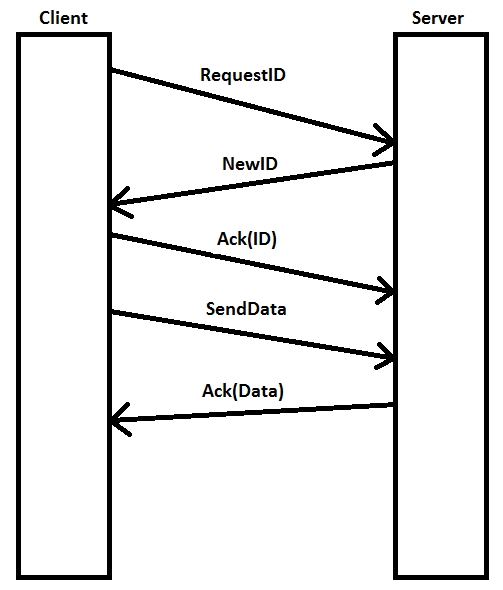
\includegraphics[width=0.4\textwidth]{figures/clientserver.png}
    \caption{Client-server illustration}
    \label{fig:clientserver}
\end{figure}

\figref{fig:clientserver} illustrates how our client-server structure works.
The client sends a RequestID command to the server.
The server responds with an ID, which is an integer that increases every time a RequestID command is received.
The reason the server provides the ID is to prevent clashes, which might occur if the clients generated the IDs.
The client sends back an acknowledgement to the server when it has received the ID.
When the client has received the ID, it then acknowledges the ID received.
The client sends the data to the server that is needed to create a new route, or gives information about the route it is following.
The server then sends an acknowledgement that it has received the data.


The messages that are sent back and forth are converted into bytes.
In \figref{fig:bytesclientserver} it is illustrated how the bytes are packed.
32 bits are reserved for our ClientID, which is empty when the first message is sent to request an ID.
Next we have our RequestID command which takes 16 bits and for the other commands\todo{List/table of commands} there is 8 bits.
We have reserved one bit as a Last message ID\todo{Layers, splitting, blabla. Skriv det, Andreas!}, which is used to be able to tell if a big message,
that is split into 2 or more files has ended.

\begin{figure}[h!]
  \centering
    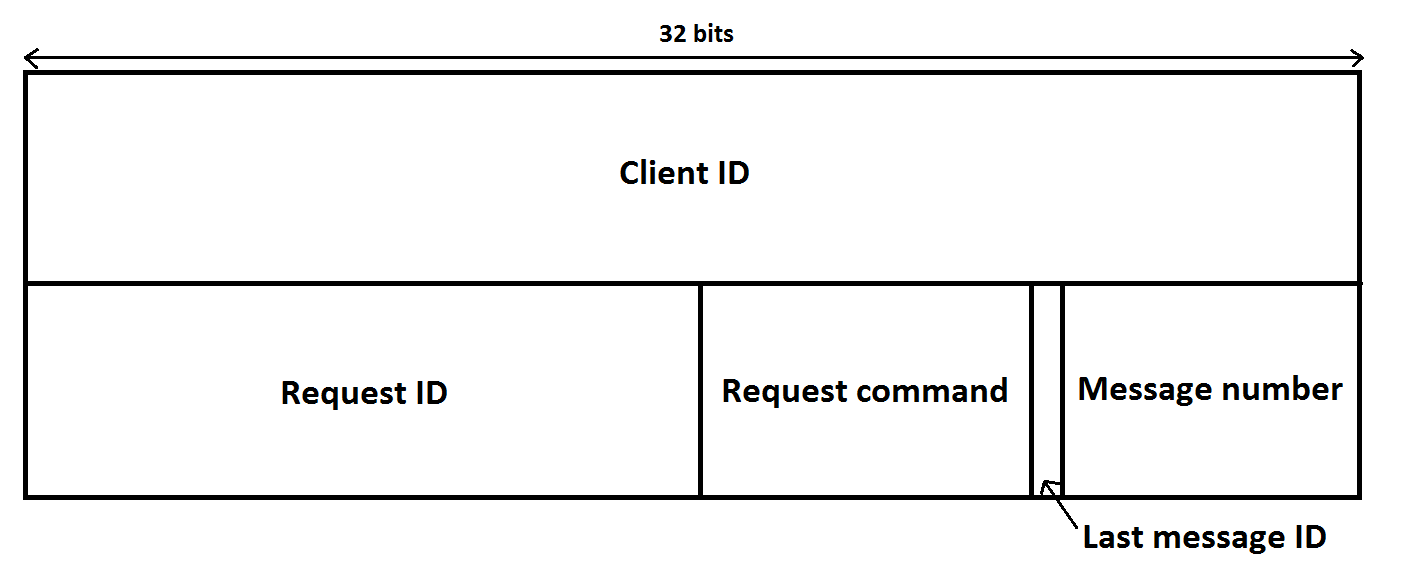
\includegraphics[width=1\textwidth]{figures/bytesclientserver.png}
    \caption{Illustration of header composition}
    \label{fig:bytesclientserver}
\end{figure}\todo{det der vi snakkede om med striberne}

The client updates its GPS location every 5 seconds, so as to be able to maintain a precise location of the client. This information, the speed, and the time is sent to the server, and can be used to learn traffic patterns.
%When a message is sent either from the client or the server,
%they are both set to wait for 5 seconds to receive the acknowledgement message, if no such message is received the message is discarded. We could have continued to try and resend the message several times, but a lost GPS coordinate from a user is not a critical problem for our system and will not have any major effect on our calculations.


On the client we have implemented an OpenStreetMap viewer and a getRoute method where the client asks for a route between two points, this is done by sending 2 node ids, node ids are explained in \secref{chap:FormatPre-processing}, to the server where then the fastest path is calculated between the 2 points. The server then sends GPS locations of the route which then is shown in the OpenStreetMap on the client. An illustration of this can be seen in \figref{fig:routeonmap}.

\begin{figure}[H]
  \centering
    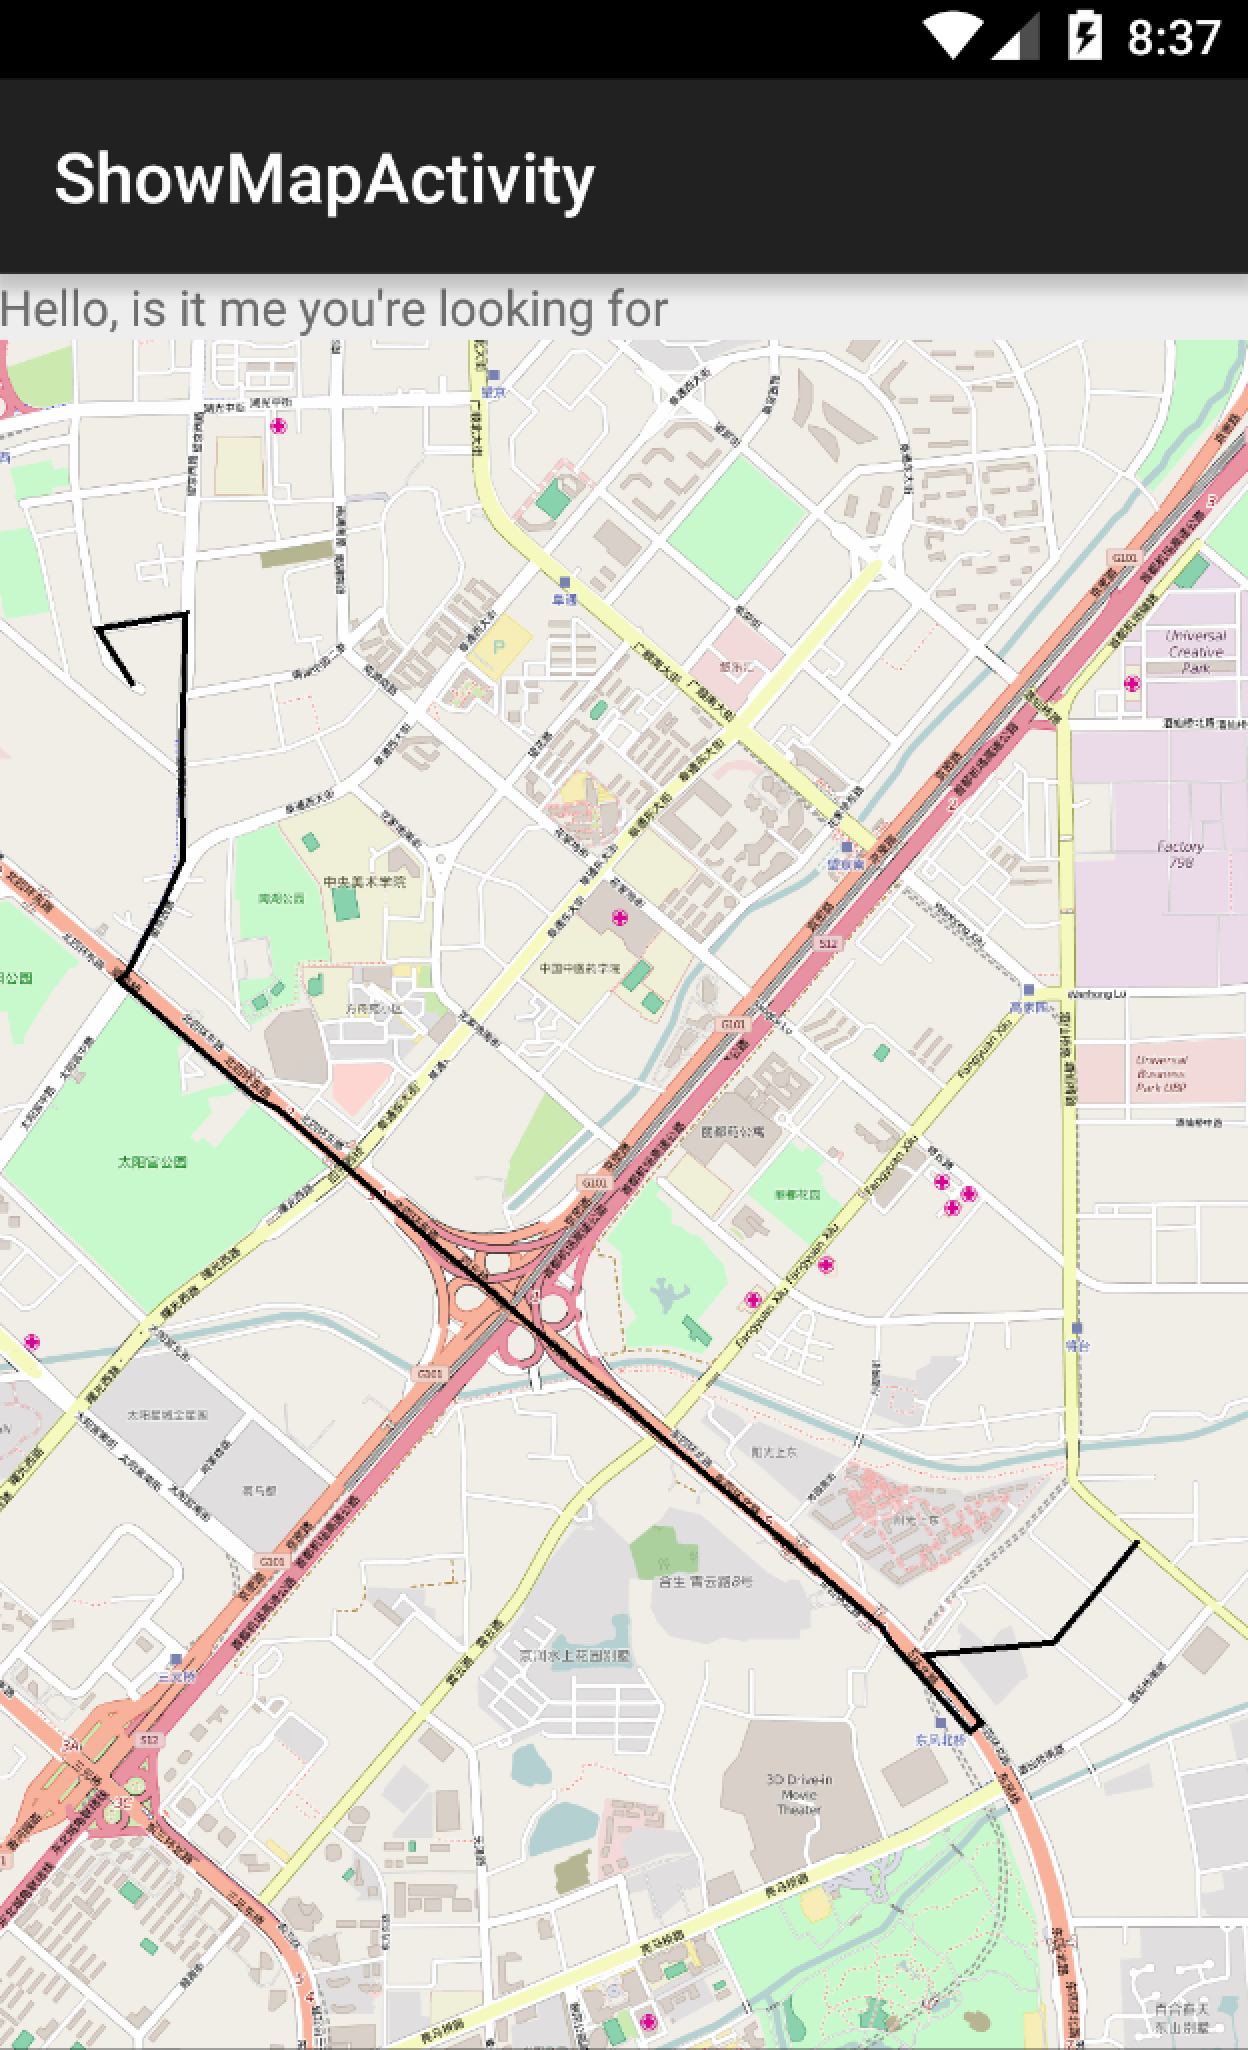
\includegraphics[width=0.6\textwidth]{figures/routeOnMap.png}
    \caption{Illustration of a route sent from the server to the client shown on an android device}
    \label{fig:routeonmap}
\end{figure}
